\documentclass{article}

\usepackage{amsmath} % math stuff
\usepackage{amssymb} % math stuff
\usepackage{array} % equations and stuff
\usepackage{bm} % bold math
%\usepackage{caption} % suppressed table numbering; incompatible with revtex, and longtable, I think
\usepackage{comment} % comment environment
%\usepackage{enumitem} % customization of enumeration, itemize, and description
\usepackage[T1]{fontenc} % font encoding for special characters, must also use scalable font package
\usepackage[margin=0.8in]{geometry} % paper sizes and margins (but be careful not to mess up pre-defined pages)
\usepackage{graphicx} % for graphics
%\usepackage{helvet} % default font is the helvetica postscript font
\usepackage{layouts} % print units like widths
\usepackage{lipsum} % lorem ipsum filler text
\usepackage{lmodern} % scalable font?
\usepackage{longtable} % multi-page tables
\usepackage{makecell} % specify line-breaks in table cells
\usepackage{mathrsfs} % math script font
\usepackage{mhchem} % easier chemical formula
\usepackage{microtype} % allows disabling of ligatures
%\usepackage{newcent} % new century schoolbook font
\usepackage{nicefrac}
\usepackage{numprint} % print and format (large) numbers
\usepackage{parskip} % removes paragraph indentation, and adjusts paragraph skip, as well as list items
\usepackage{pdfpages} % add pdf files as pages
%\usepackage{setspace} % adjust text spacing and indents
\usepackage{siunitx} % decimal alignment
\usepackage{subfigure} % divided figures
%\usepackage{tabu} % extra table options
\usepackage{textcomp} % symbols
\usepackage{threeparttablex} % better footnotes with longtable
\usepackage{titling} % title placement
\usepackage{ulem} % strikethrough text
%\usepackage{url} % superceded by hyperref
\usepackage{verbatim} % verbatim environment
\usepackage{xcolor} % colors and color boxes
\usepackage{xspace} % commands that don't eat up white space
\usepackage{hyperref} % links and page setup; should always come last

\hypersetup{
 bookmarks=true,
 colorlinks=true,
 citecolor=blue,
 linkcolor=blue,
 urlcolor=blue,
 pdfstartview={XYZ null null 1.0} % default open view is 100%
}

\DisableLigatures[f,t]{encoding = T1} % disable ff, fi, fl, tt ligatures, without f option, it also disables -- = endash
\renewcommand{\arraystretch}{2.0} % extra vertical space in tables

\begin{document}

\pagestyle{empty} % don't number pages

% custom title
\begin{center}
{\LARGE Express Riddler}

\vspace{0.15in}

{\Large 29 January 2021}
\end{center}


\section*{Riddle:}

I recently found four cubic blocks in a peculiar arrangement.
Three of them were flat on the ground, with their corners touching and enclosing an equilateral triangle.
Meanwhile, the fourth cube was above the other three, filling in the gap between them in a surprisingly snug manner.
Here's a photo I took of this arrangement:

\vspace{0.1in}
\begin{center}
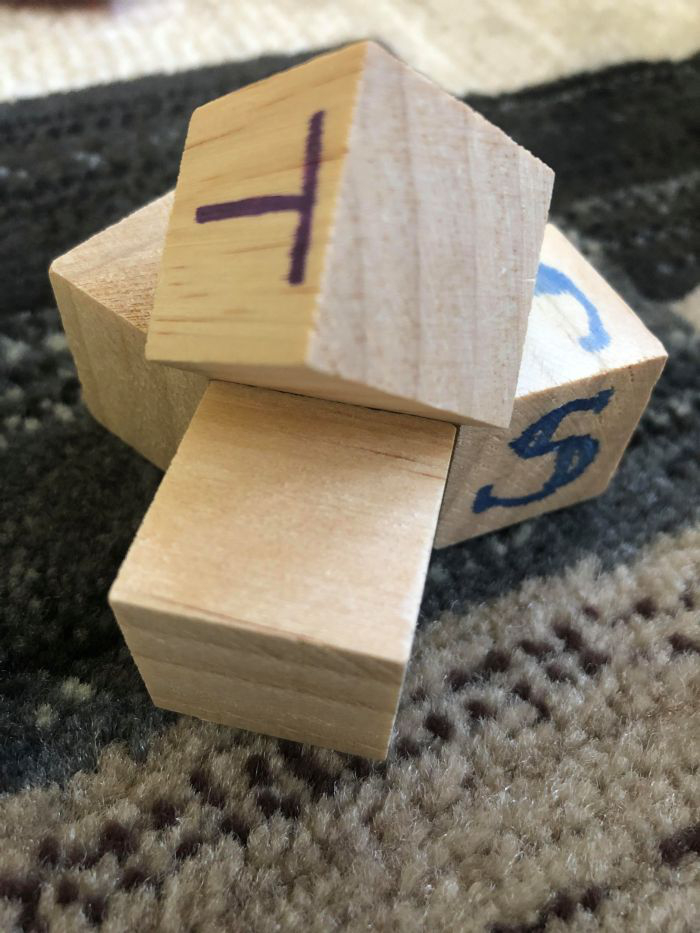
\includegraphics[width=2.5in]{four_cubes.jpg}
\end{center}
\vspace{0.1in}

If you too have blocks at home (I mean, of course you do), see if you can make the same arrangement.

Now, if each of the four cubes has side length 1, then how far above the ground is the bottommost corner of the cube on top?

\section*{Solution:}

Here are the three (not-quite-to-scale) diagrams I used to solve this geometric problem:

\vspace{0.2in}
\begin{center}
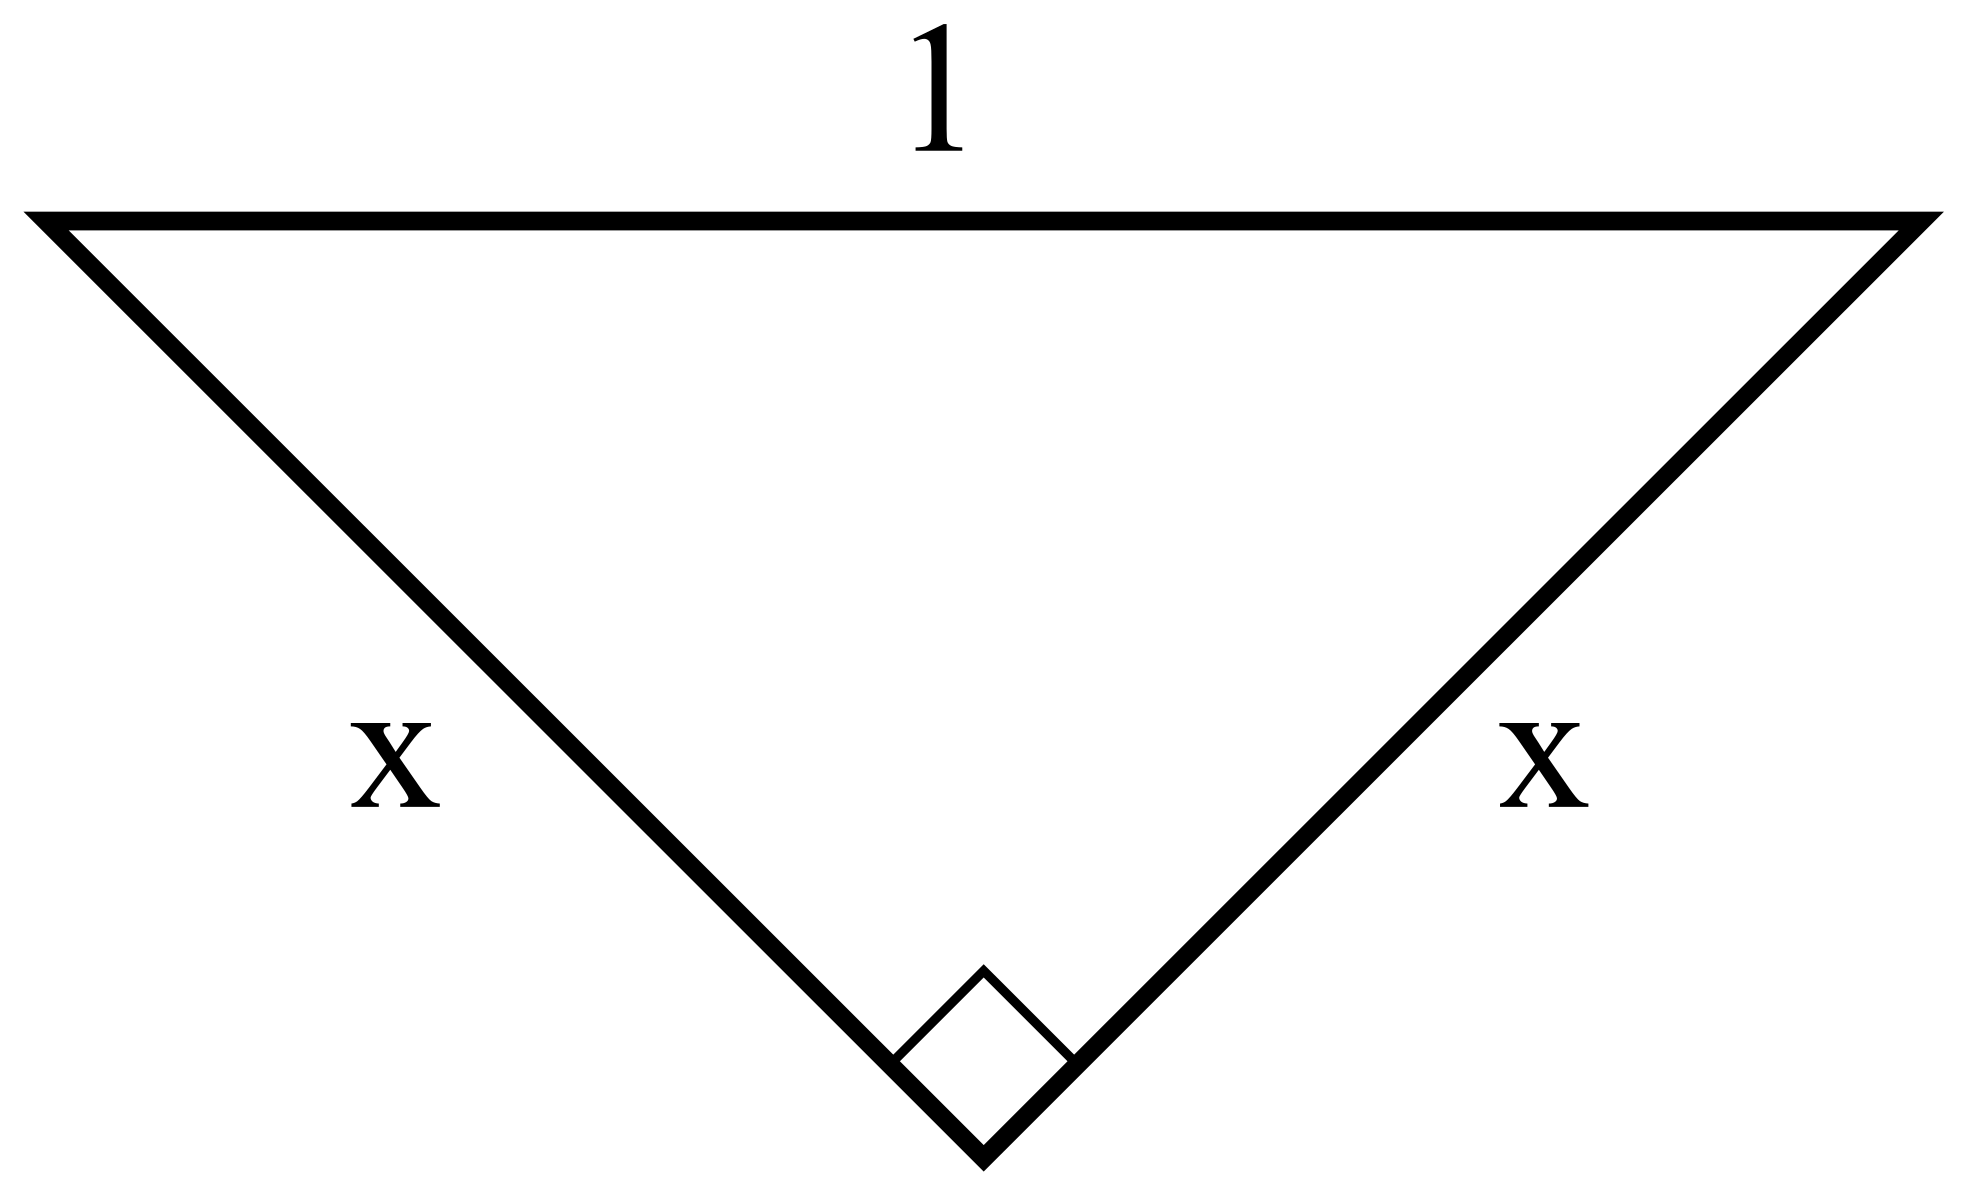
\includegraphics[width=2in]{triangle1.png}
\quad
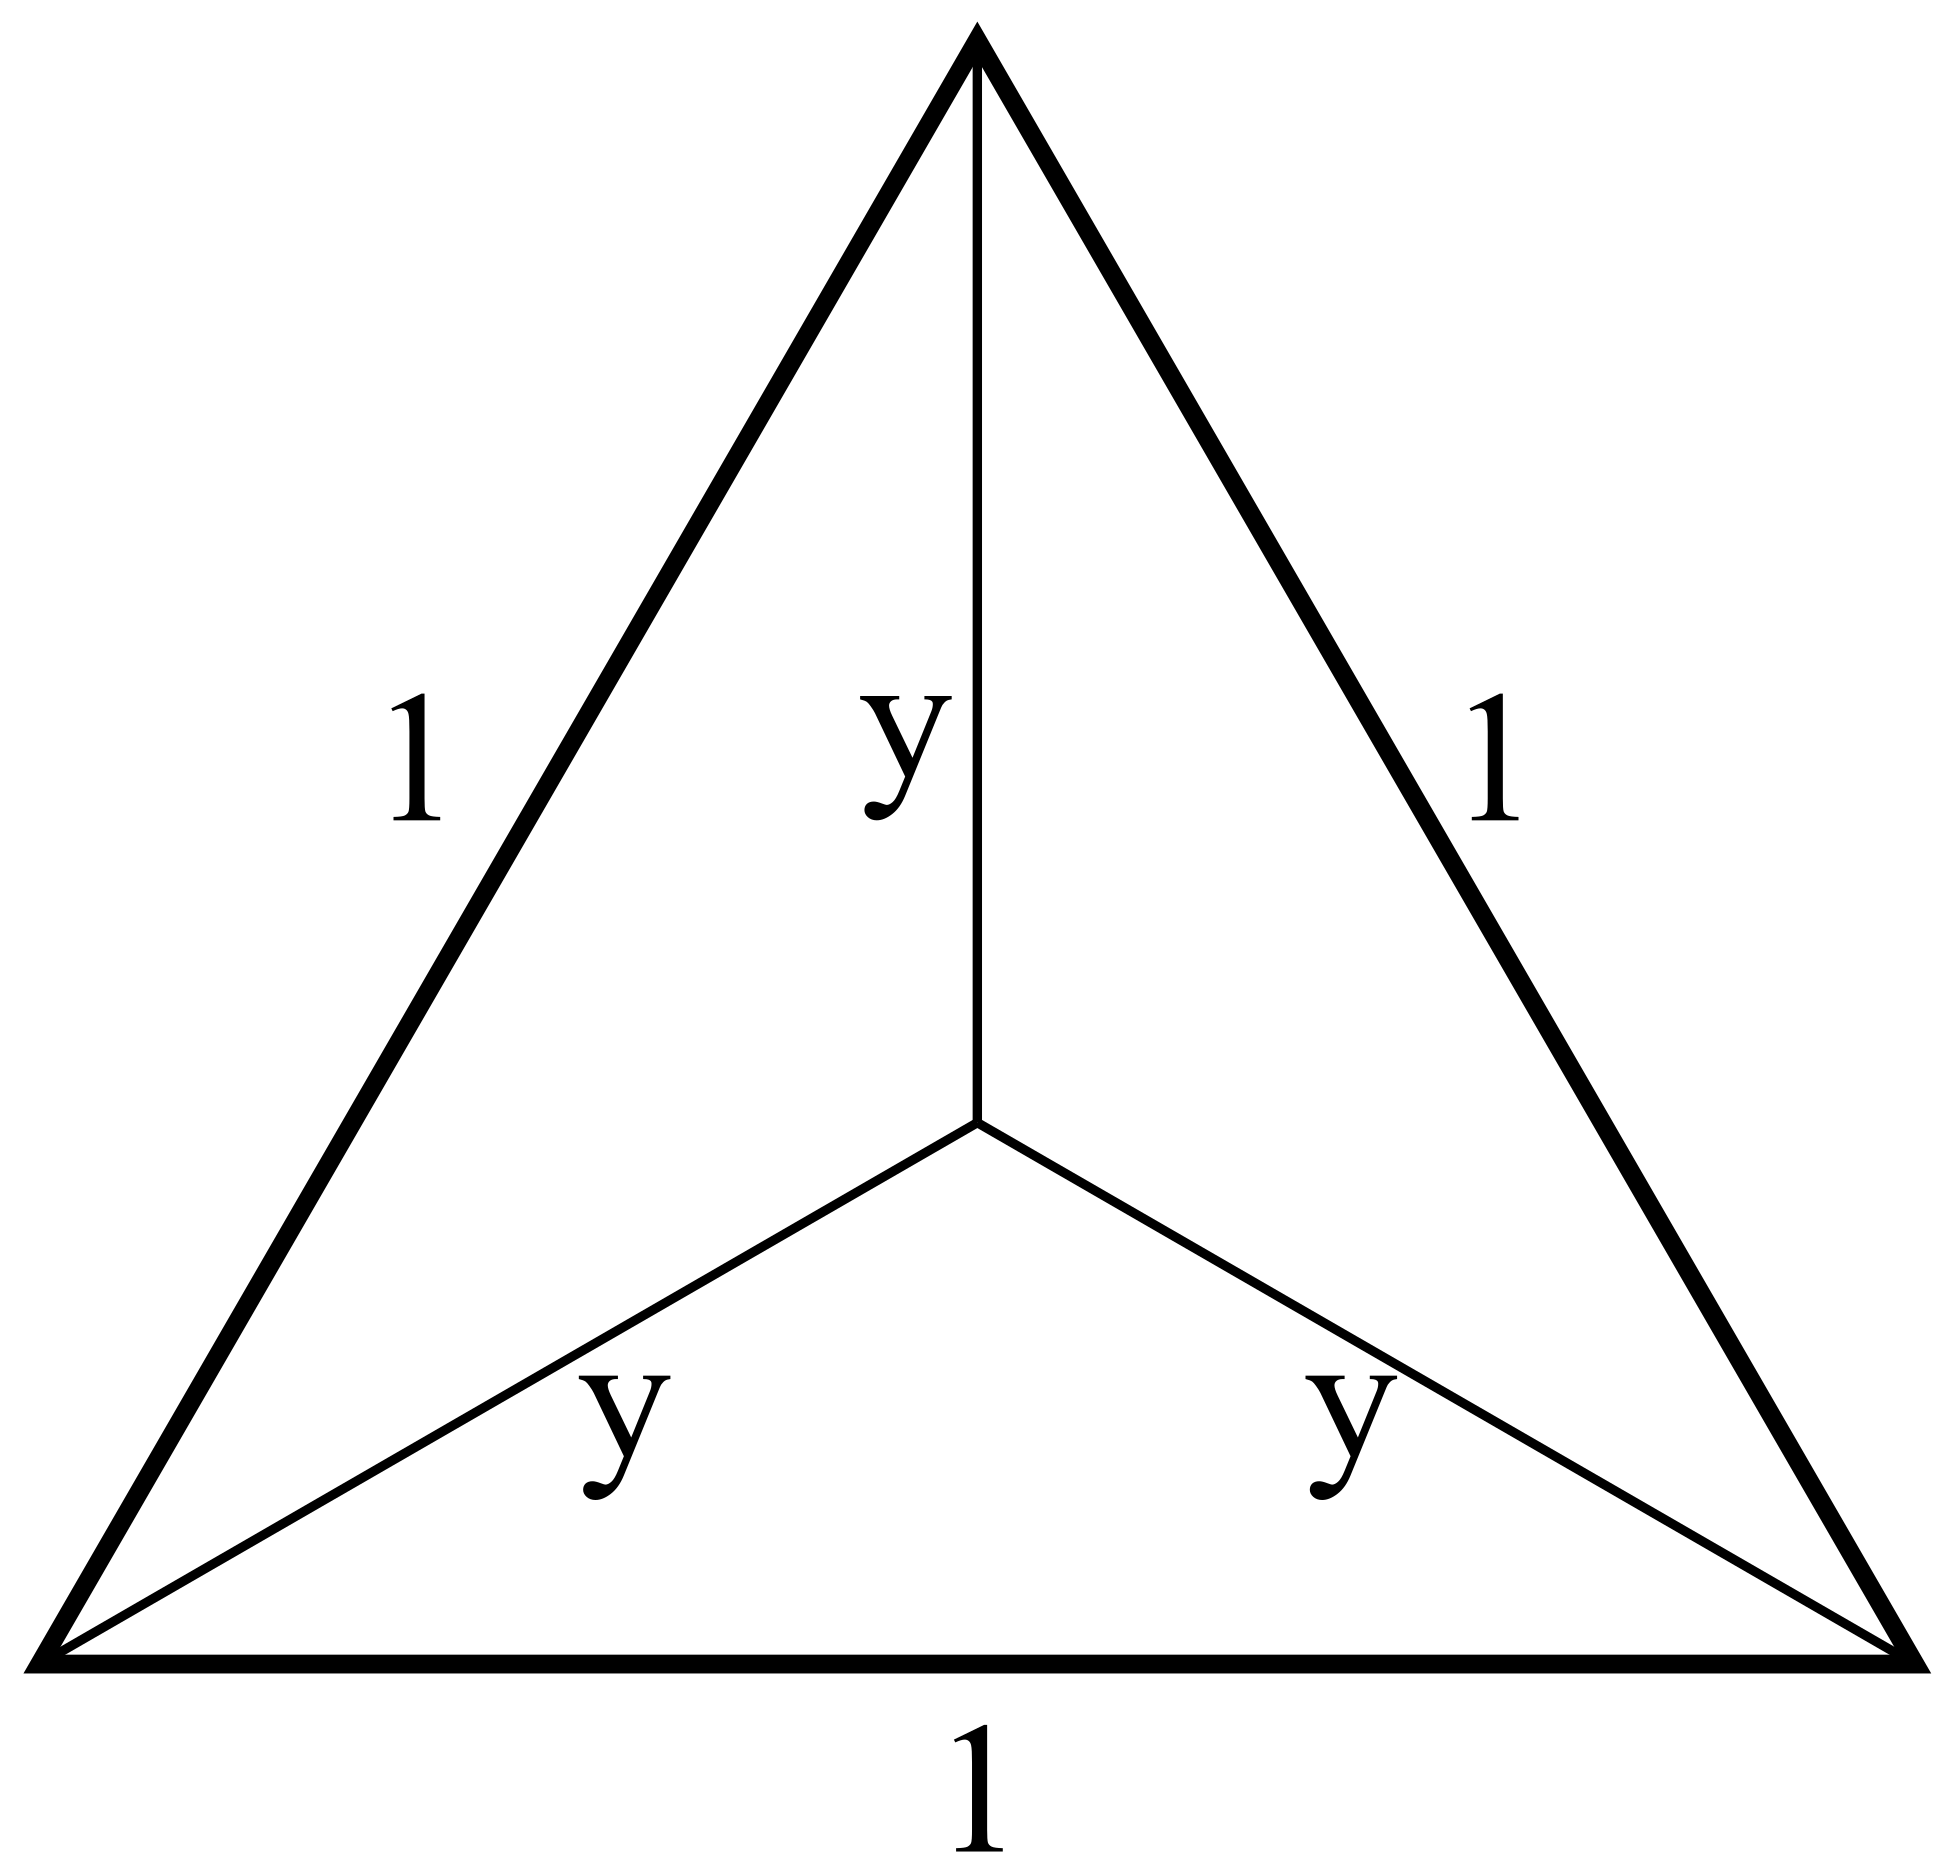
\includegraphics[width=2in]{triangle2.png}
\quad
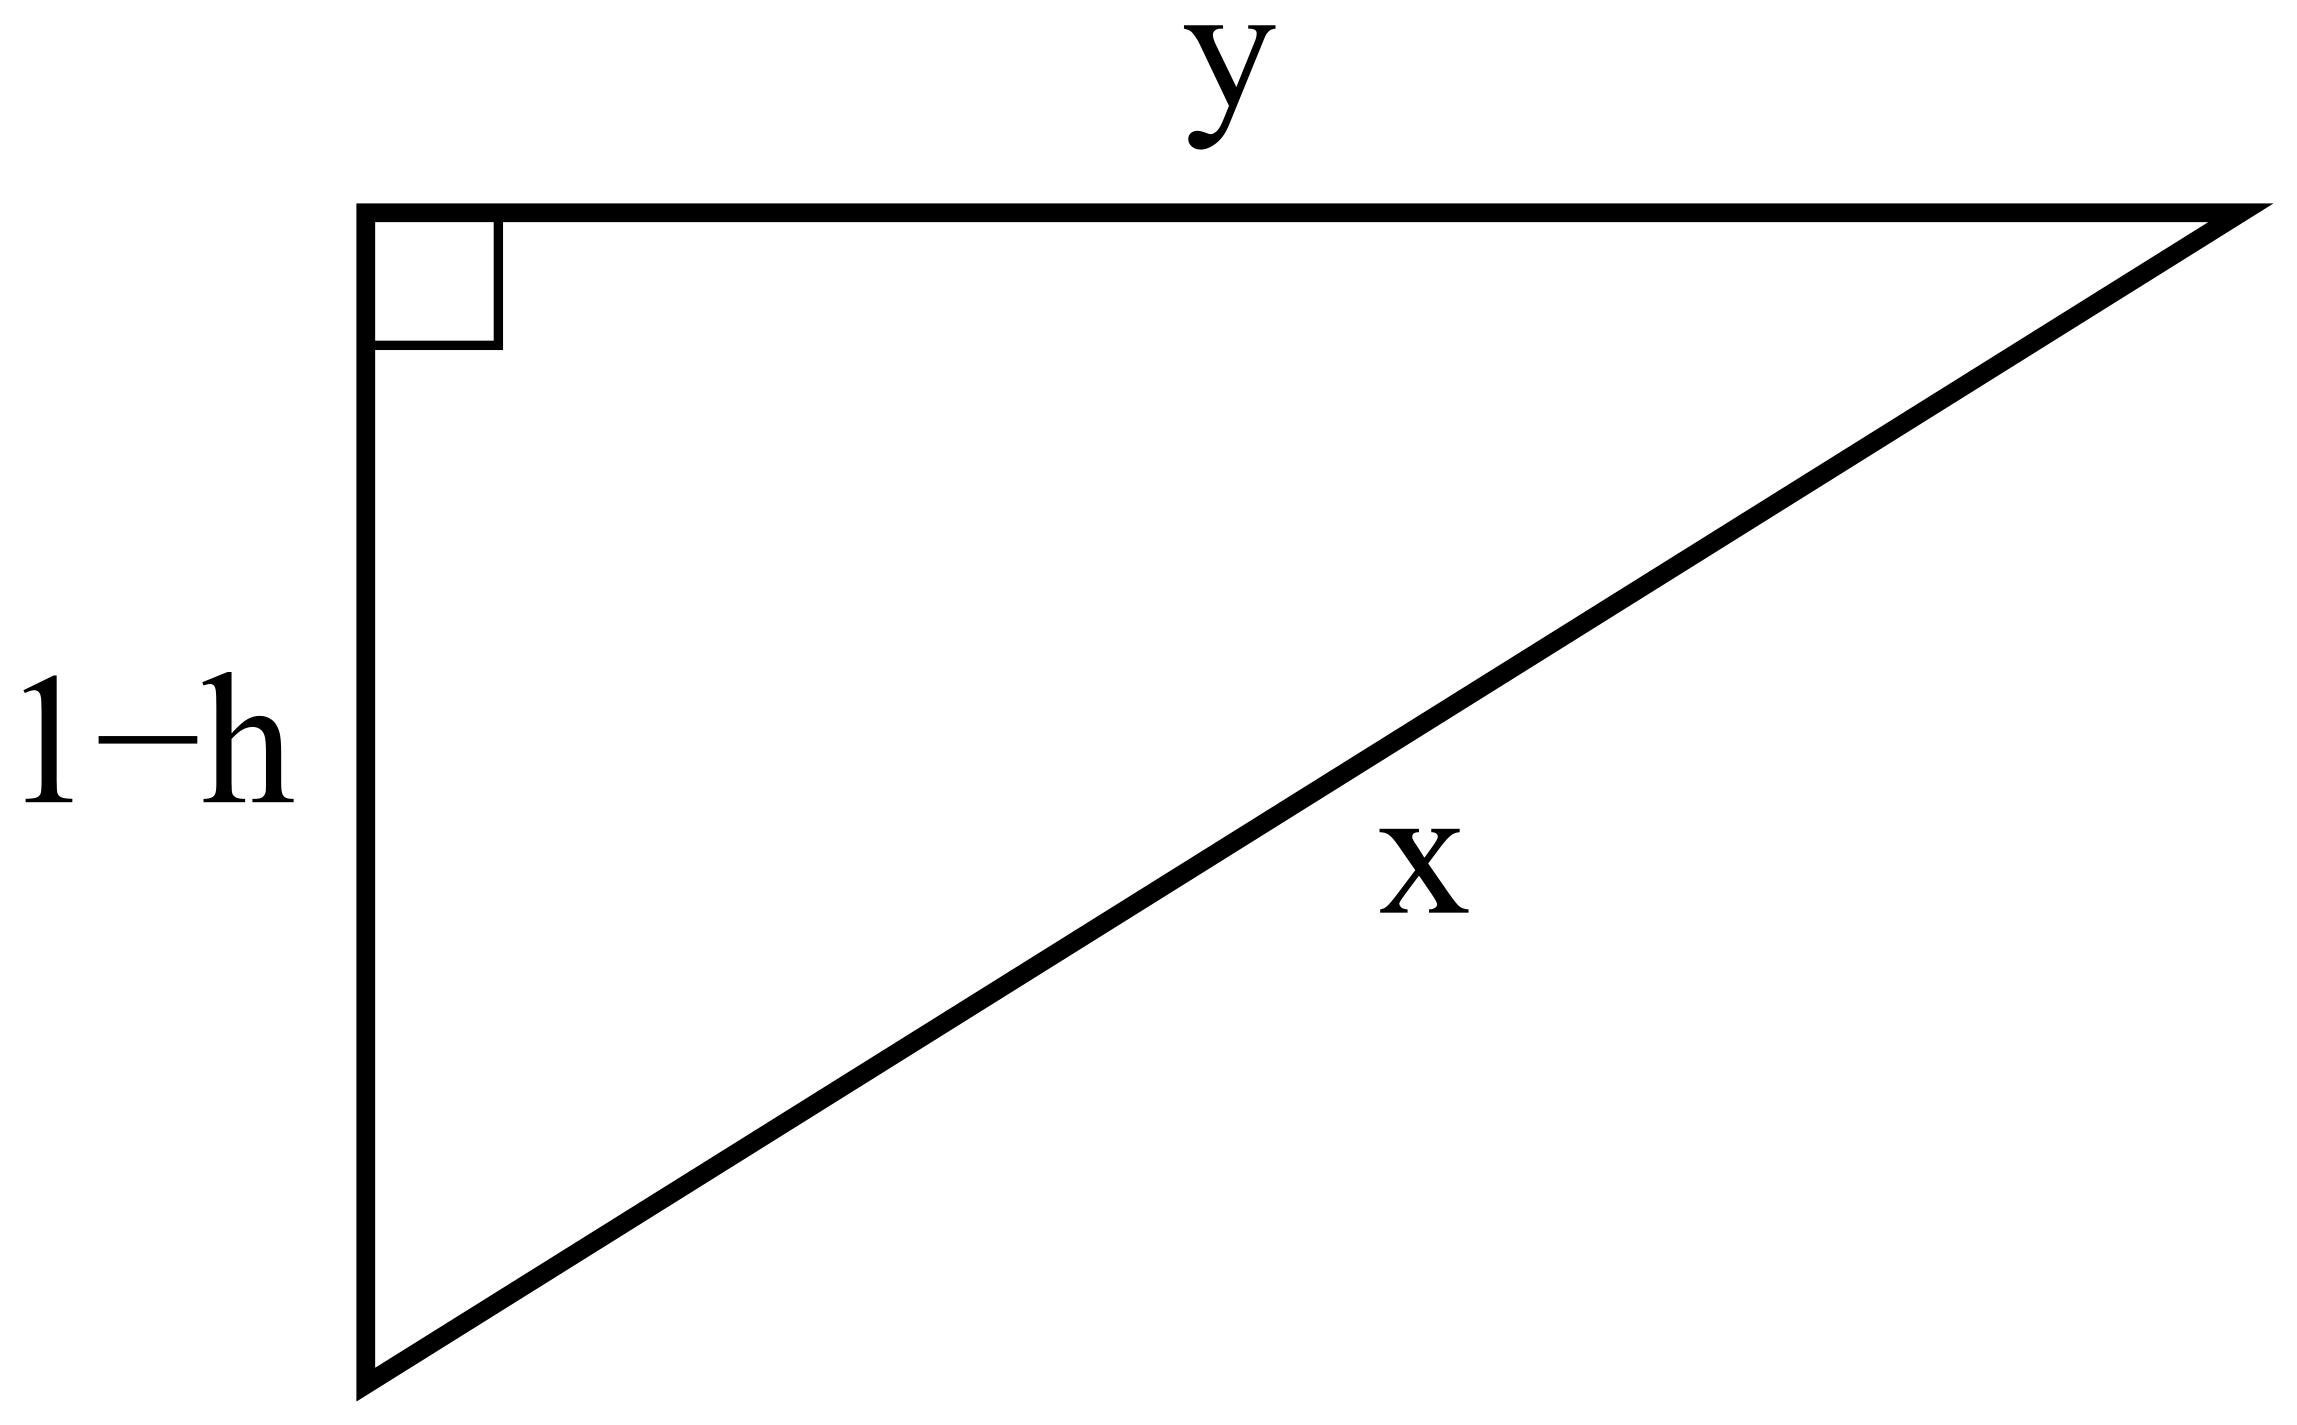
\includegraphics[width=2in]{triangle3.png}
\end{center}
\vspace{0.3in}

The left-most triangle is the section of each of the three faces of the upper cube which dips down into the other cubes.
It is a right triangle pointing downward and sitting at the bottom vertex.
The hypotenuse of length 1 is flush with an edge of an outer cube.
The length $x$ is the length of one of the upper cube's edges which lies inside the other cubes.
It is almost trivial to show that $x=\nicefrac{\sqrt{2}}{2}$.

The middle triangle is either a cross-section or a ``shadow'' of the upper cube along the horizontal plane.
It is an equilateral triangle whose three sides of length 1 are the edges of each of the outer cubes.
The lengths $y$ are formed by the shadows of each $x$ which meet in the center of the triangle.
With a bit more geometrical calculations, it can be shown that $y=\nicefrac{\sqrt{3}}{3}$.

Finally, the right-most triangle shows how each edge $x$ dips down inside the outer cubes.
From the top plane of ther outer cubes, the cube's bottom vertex is a distance $1-h$ down, leaving the remaining $h$ as the distance from the bottom plane.
Based on the other values determined above, the value of $h$, and the riddle's solution, is
\fcolorbox{red}{white}{$\bm{{1-\nicefrac{\sqrt{6}}{6}\approx0.592}}$}\,.



\end{document}